%Model Presentation: detailed  presentation of a model, including justifications for design decisions

The presentation of our solution to the \mpc follows a systematic methodology where modeling choices are introduced step by step, as the requirements are stated. Satisfaction of requirements is explained throughout this presentation.

%\todo[inline]{phrase d'intro pour expliquer que les req étaient couverts au fur et à mesure (côté systématique)}

The designed multilevel architecture shown in Figure~\ref{fig:MultilevelArchitecture} captures the two use cases described in the Process Challenge.

% Expliquer que le use case XSure ne nécessitait pas l'extension de metamodèle requise pour le usecase Acme Software Developement Process

\subsection{Base metamodel for the Process Challenge}

\begin{figure*}
 \centering
    % 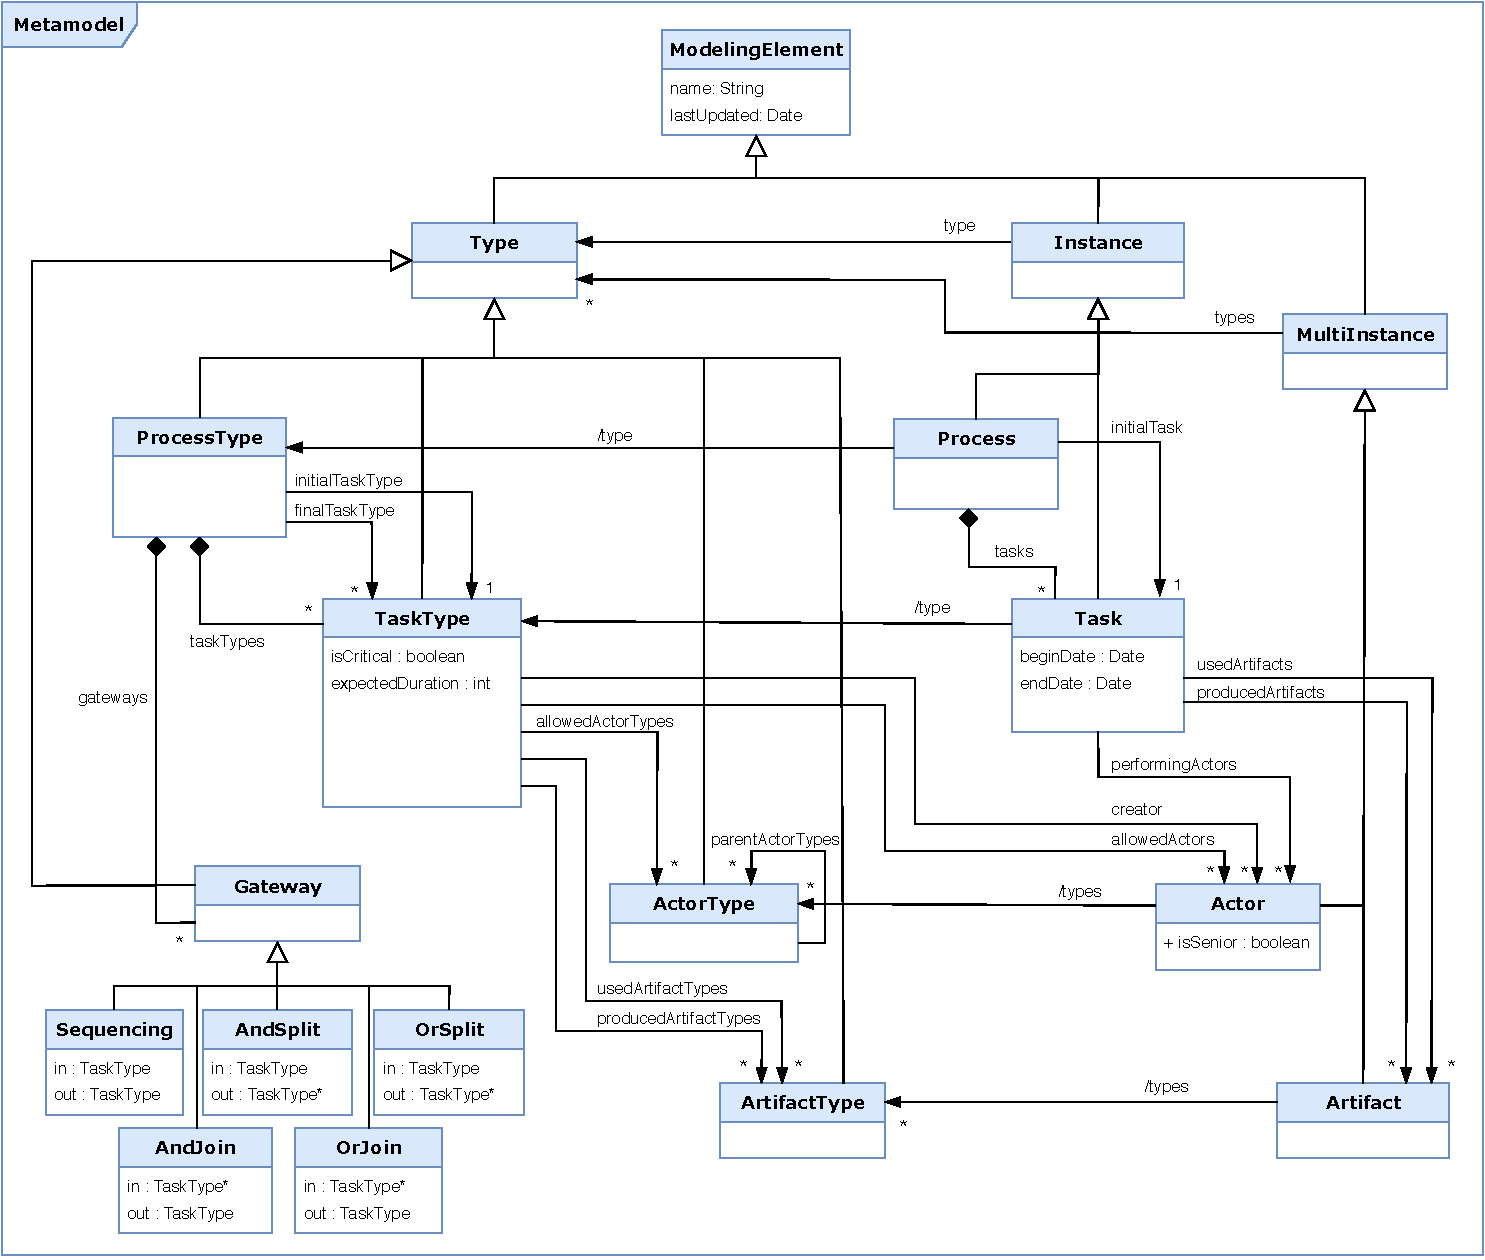
\includegraphics[width=1.0 \columnwidth]{Figures/Metamodel.pdf}
    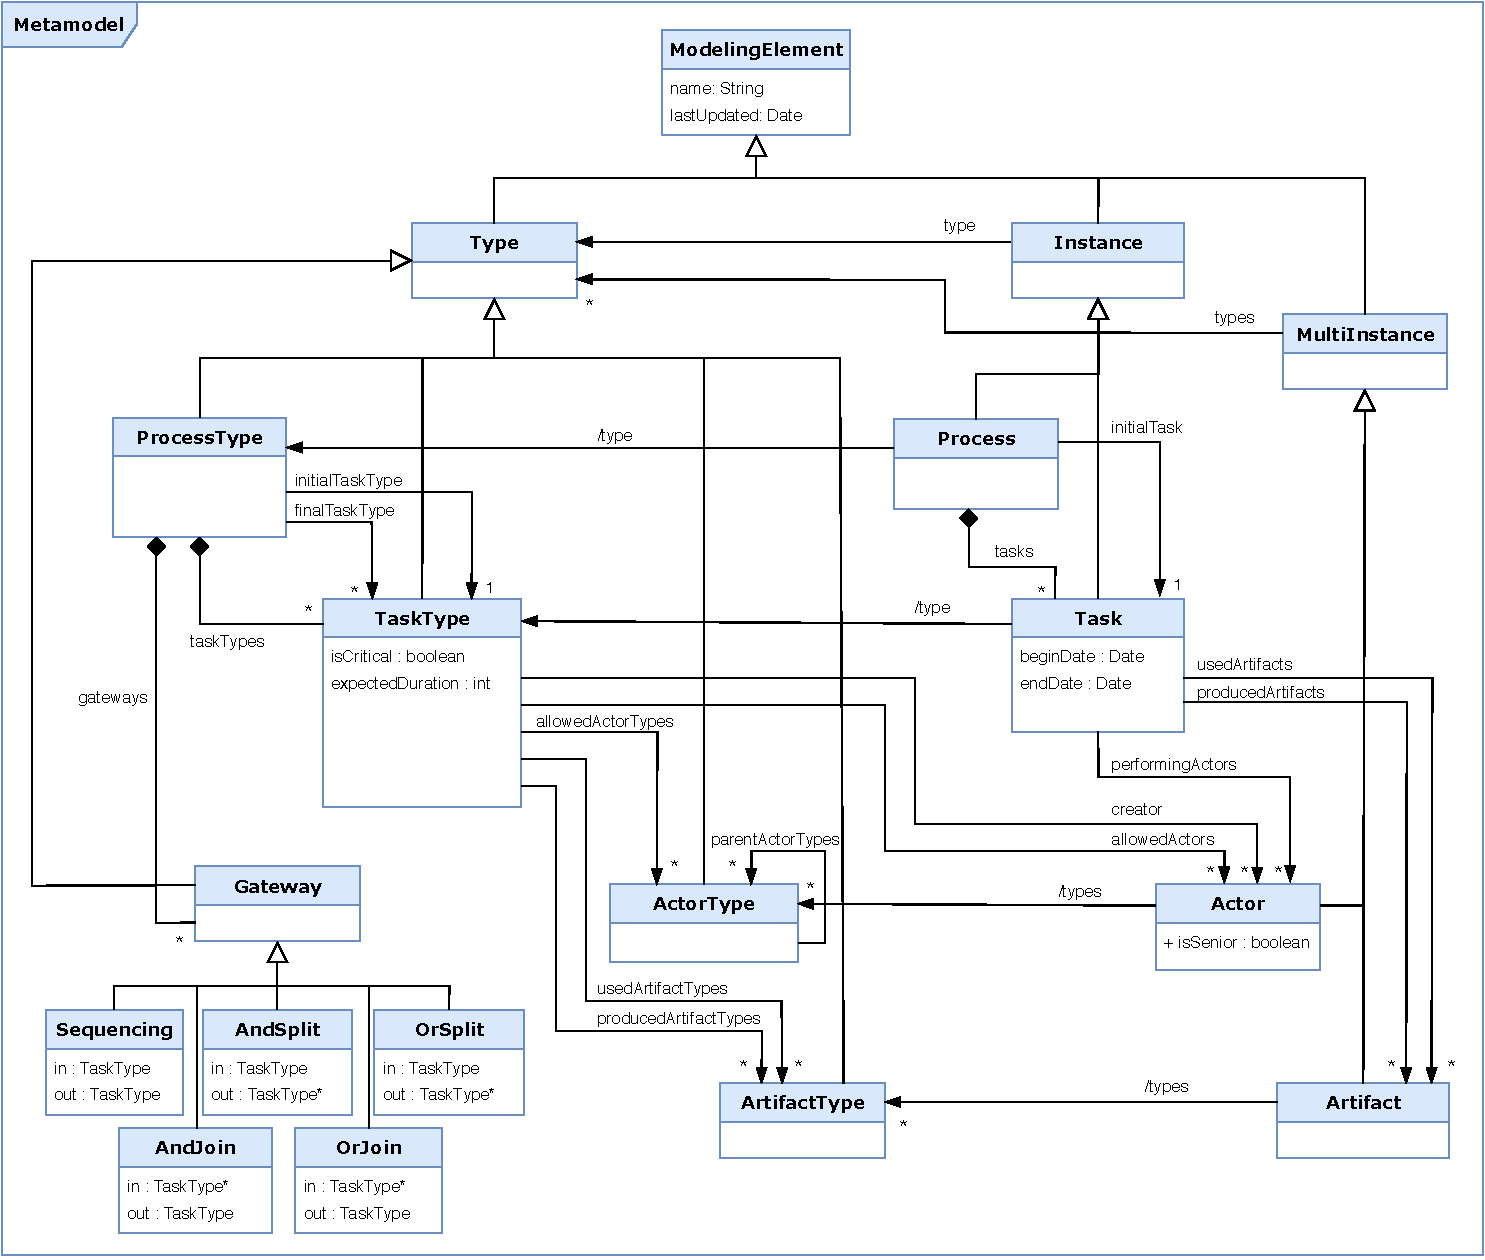
\includegraphics[width=1.0 \textwidth]{Figures/Metamodel.pdf}
     \caption{Process management base metamodel}
    \label{fig:BaseMetamodel}
\end{figure*}

In this section, we present the base metamodel presented in figure~\ref{fig:BaseMetamodel} with \textit{XSure} insurance domain use case, whose partial description was provided in the challenge description. The requirements \textbf{P1} to \textbf{P19} of XSure insurance domain are straightforwardly implemented by instantiating the \emph{XSure model}, as an instance of base metamodel (the left side of figure~\ref{fig:MultilevelArchitecture}).

Figure~\ref{fig:BaseMetamodel} represents this base metamodel with a \UML-like formalism, well adapted to represent \FML concepts and their instances. A \textit{Concept} of \FML is represented by a \UML class where roles of basic types are attributes. The roles whose types are concepts are represented by a combination of a name in their containing concept and an arrow from their name to their type. The cardinality follow the \UML practice.
For example, the role \texttt{parentActorTypes} of the concept \texttt{ActorType} has the type \texttt{ActorType} and the * cardinality.

Our proposition relies on ontologic instantiation as presented in figure \ref{fig:LinguisticAndOntologicInstantiation}, with a common root concept \texttt{ModelingElement}. Two types of ontological instantiation are needed to meet the requirements of the challenge. One provides that some instances conform to only one type (\texttt{Process} and \texttt{Task} do respectively conform to \texttt{ProcessType} and \texttt{TaskType}). While some entities define their conformity to several types (\texttt{Actor} and \texttt{Artifact} do respectively conform to several \texttt{ActorType} and \texttt{ArtifactType}). These instantiations are respectively expressed using the relations \texttt{type} and \texttt{types} between \texttt{Type}, \texttt{Instance} and \texttt{MultiInstance} concepts. In the diagram, the realization of these relations are indicated by a derived relation, \texttt{/type} or \texttt{/types}, as for example between \texttt{Process} and \texttt{ProcessType} or between \texttt{Actor} and \texttt{ActorType}.

\subsubsection{Process type definition}

We first present the process definition part of base metamodel, located left of figure \ref{fig:BaseMetamodel}.

% Illustrer avec des instances de XSure

\texttt{ProcessType} is a specialization of the \texttt{Type} concept, and references a collection of \texttt{TaskType} through the composition relation \texttt{taskTypes} with (0..*) cardinality (\textbf{P1}). A \texttt{TaskType} is embedded in a \texttt{ProcessType} and inherits from its context. To illustrate this in \textit{XSure} insurance domain use case, \textit{XSure model} defines \textsf{Claim Handling}, instance of \texttt{ProcessType}, and \textsf{Receive Claim}, \textsf{Assess Claim} and \textsf{Pay premium}, instances of \texttt{TaskType}.

\texttt{ProcessType} also references a collection of gateways, reified with the \texttt{Gateway} concept hierarchy. \texttt{Gateway} is a specialization of \texttt{Type} and is specialized by \texttt{Sequencing}, \texttt{AndSplit}, \texttt{AndJoin}, \texttt{OrSplit} and \texttt{OrJoin} concepts (\textbf{P2}). Depending on its type and following its underlying operational semantics, a gateway defines one or more inputs and one or more outputs. A \texttt{ProcessType} additionally exposes a unique initial \texttt{TaskType} and a collection of final \texttt{TaskType} with both roles \texttt{initialTaskType} (single cardinality) and \texttt{finalTaskType} (cardinality 0..*) (\textbf{P3}). \textt{TaskType} exposes a creator role as a reference to an \texttt{Actor} concept (\textbf{P4}), which is at the same conceptual level. 

The following listing shows an excerpt of the \FML code modeling some core concepts of process modeling base metamodel. 

\begin{lstlisting}
model MetaModel {

  concept ModelingElement { ... }
  
  concept Type extends ModelingElement { ... }
  
  concept ProcessType extends Type {
    TaskType[0..*] taskTypes;
    TaskType initialTaskType;
    TaskType[0..*] finalTaskTypes;
    Gateway[0..*] gateways;
        
    concept TaskType extends Type {
      Actor creator;
      Actor[0..*] allowedActors;
      ActorType[0..*] allowedActorTypes;
      ...
    }
        
    abstract concept Gateway extends Type {
      abstract void execute(Process process);
      ...
    }
        
    concept Sequencing extends Gateway {
      TaskType in;
      TaskType out;
    }
    
    // Other core concepts
  }
}    
\end{lstlisting}


The \texttt{ActorType} concept is a sub-concept of \texttt{Type} and the \texttt{allowedActorTypes} relation to \texttt{ActorType} defined in \texttt{TaskType} (with 0..* cardinality) captures \textbf{P5} requirement. Requirement \textbf{P6} is symmetrically satisfied with \texttt{allowedActors} relation to \texttt{Actor} also defined in \texttt{TaskType} (with 0..* cardinality). The same modeling pattern applies to \texttt{ArtefactType} defined as a sub-concept of \texttt{Type}, and both relations \texttt{usedArtifactTypes} and \texttt{producedArtifactTypes} defined in \texttt{TaskType} (\textbf{P7}). \texttt{TaskType} additionally exposes an \texttt{expectedDuration} role (expressed in number of days), satisfying \textbf{P8}.
\noteFabien{expectedDuration pas dans la figure}

The \texttt{Actor} concept defines a boolean attribute called \texttt{isSenior}, while \texttt{TaskType} defines an additional \texttt{isCritical} boolean attribute, indicating that some instance are flagged as critical and must be performed by senior actors. To fulfil \textbf{P9} requirement, a supplementary constraint is required for \texttt{TaskType} and is captured through the following invariant expressed in the \FML language:

\begin{lstlisting}
forEach (actor : allowedActors) {
    assert !isCritical | actor.isSenior
}
\end{lstlisting}

This invariant should be completed with additional constraints defined in the \texttt{Task} concept, which apply to performing actors assigned to enact tasks. 

\todo{Gérer également la fin de P9, non traité pour le moment: artifact they produced must be associated with a validation task}

\subsubsection{Process enactment}
\label{sec:ProcessEnactment}
We now present the process enactment part of base metamodel, located right of figure~\ref{fig:BaseMetamodel}. All concepts defined in this subsection are either specialization of the \texttt{Instance} concept (if they have exactly one type) or the \texttt{MultiInstance} concept (when they have several types).

\texttt{Process} represents an enacted \texttt{ProcessType}, as defined in previous subsection (\textbf{P10}). FML defines behavioral features called behavior. \texttt{ProcessType} defines the behavior \texttt{newProcess(String)}, taking the name of the process to enact as argument:

\begin{lstlisting}
public Process newProcess(String name) {    
  Process newProcess = new Process(name,this);  
  for (taskType : taskTypes) {      
    Task newTask = taskType.newTask(newProcess.name+"-"+taskType.name),newProcess);        
  }      
  return newProcess;    
}    
\end{lstlisting}

This scheme rely on \FML dynamic binding mechanism to delegate to task types the responsibility of instances creation. An instance of \texttt{Process} references its unique type \texttt{ProcessType} by the specialized \texttt{/type} role. Each instance of \texttt{TaskType} is ontologically instantiated with a \textit{Task} (\textbf{P11}), using the same pattern where \textit{TaskType} has the responsability to manage this ontological instantiation. A \textit{Task} references its unique \textit{TaskType}, and defines a \textit{begin date} and an \textit{end date} as basic attributes of the concept (\textbf{P12}).

Same pattern applies for artifacts used and produced with roles \textit{usedArtifacts}, \textit{producedArtifacts} and \textit{performingActors} defined in \textit{Task} concept (\textbf{P13}). An instance of \textit{Artifact}, defined as a specialization of \textit{MultiInstance} concept, references a set of \textit{ArtifactType} through the specialized \textit{/types} role (\textbf{P14} and \textbf{P16}). Likewise, concept \textit{Actor} is defined as a specialization of \textit{MultiInstance} concept and references a set of \textit{ActorType} through the specialized \textit{/types} relation (\textbf{P15}).

Semantics is unclear relatively to instantiation policy for artifacts. We assume that task execution implies that for each used and produced \textit{artifact type} defined in related \textit{task type}, it exists at least one \textit{artifact} declaring required ontologic instantiation (through \textit{type} role). Following excerpt of FML code shows partial implementation of this. Same patterns applied for produced artifacts.

\begin{lstlisting}
concept Task extends Instance {
  ...
  boolean declaresRequiredUsedArtifacts() {
    for (artifactType : type.usedArtifactType) {
      boolean found = false;
      for (artifact : usedArtifacts) {
        if (artifact.isOfType(artifactType))
          found = true;
      }
      if (!found) return false;
    }
    return true;
  }
  ...
}    
\end{lstlisting}

Authorization for an actor to perform a task (\textbf{P17}) is captured either through the roles \textit{allowedActors} and \textit{allowedActorTypes} defined in \textit{TaskType}. This mechanism is completed by following behaviors \textit{isAuthorizedActor(Actor)}, \textit{isValidActor(Actor)} and \textit{isValidActorType(ActorType)} defined in \textit{TaskType} : 

\begin{lstlisting}
concept TaskType extends Type {
 ...
 // Check that an Actor is authorized to perform a task, using allowed Actor and ActorTypes
  boolean isAuthorizedActor(Actor actor) {      
    for (actType : allowedActorTypes) {        
      if (actor.hasActorType(actType))         
        return this.isValidActorType(actType);          
    }        
    for (act : allowedActors) {        
      if (actor == act)         
        return this.isValidActor(actor);
    }
    return false;
  }
  
 // Check that an Actor may perform this TaskType (override when required)
  boolean isValidActor(Actor actor) {
    return true;
  }

 // Check that an ActorType may perform this TaskType (override when required)
  boolean isValidActorType(ActorType actorType) {
    return true;
  }
  ...
}
\end{lstlisting}

\textit{Task} concept basically delegates this authorization to its related \textit{TaskType}, as shown in following FML excerpt:

\begin{lstlisting}
concept Task extends Instance {
  ...
  boolean isAuthorizedActor(Actor actor) {      
    return type.isAuthorizedActor(actor);      
  }
  ...
}
\end{lstlisting}

Enforcing those constraints is finally performed by the definition of this invariant in \textit{Task} concept:

\begin{lstlisting}
forEach (actor : performingActors) {
  assert isAuthorizedActor(actor);
}
\end{lstlisting}

Default behavior states that all actors and actor types are valid for all task types. This modeling scheme offers many extension points, by the redefinition of one or some behaviors in inherited concepts (although none were required in the context of XSure insurance use case).

Actor types specialization is captured by the \textit{parentActorTypes} relation defined in \textit{ActorType} (\textbf{P18}). This is completed by both the definition of \textit{hasActorType(ActorType)} behavior in \textit{Actor} concept and recursive behavior \textit{isOrSpecializes(ActorType)} in \textit{ActorType}:

\begin{lstlisting}
concept ActorType extends Type {
  ActorType[0..*] parentActorTypes;
  ...
  boolean isOrSpecializes(ActorType actorType) {    
    if (actorType == this)   
      return true;      
    for (p : parentActorTypes) {      
      if (p.isOrSpecializes(actorType)
        return true;
    }
    return false;
  }
  ...
}

concept Actor extends MultiInstance {
  ...
  boolean hasActorType(ActorType actType) {      
    for (type : types) {
      if (type.isOrSpecializes(actType))
        return true;
    }
    return false;
  }     
  ...
}
\end{lstlisting}

All concepts inherits from \textit{ModelingElement}, which defines a \textit{lastUpdated} attribute with \textit{Date} type, and thus satisfies \textbf{P19} requirement. 

\subsection{The Acme software development process}
\label{sec:AcmeSoftwareDevelopmentProcess}

The challenge describes in a second part a Software engineering process for a fictional Acme company. Base metamodel as described in previous section is too generic to capture all domain-specific aspects of this use case. We choose to complete the architectual hierarchy with a specific VirtualModel, specific to Acme software development process metamodel, as shown in figure \ref{fig:AcmeArchitecture}. \textit{Acme} metamodel inherits and specializes base metamodel, and \textit{Acme model} is defined as an instance of \textit{Acme} metamodel. The metamodel inheritance is implemented as VirtualModel's inheritance. Any instance of Acme model is either an instance of a concept defined in base metamodel, or a concept defined in specialized Acme metamodel, which may or not inherit from a concept defined in base metamodel.
% FML follows a classical object-oriented semantics. ???

\begin{figure}
 \centering
    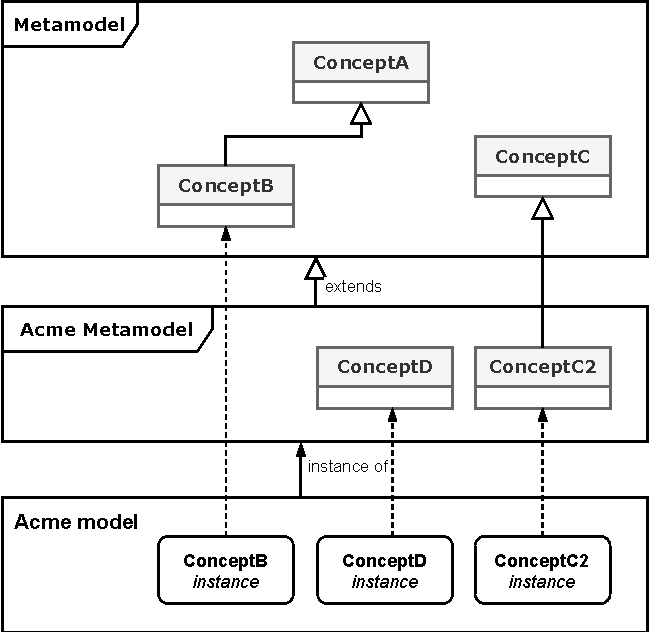
\includegraphics[width=1.0 \columnwidth]{Figures/AcmeArchitecture.pdf}
     \caption{Acme software development process architecture}
    \label{fig:AcmeArchitecture}
\end{figure}

\begin{figure*}
 \centering
     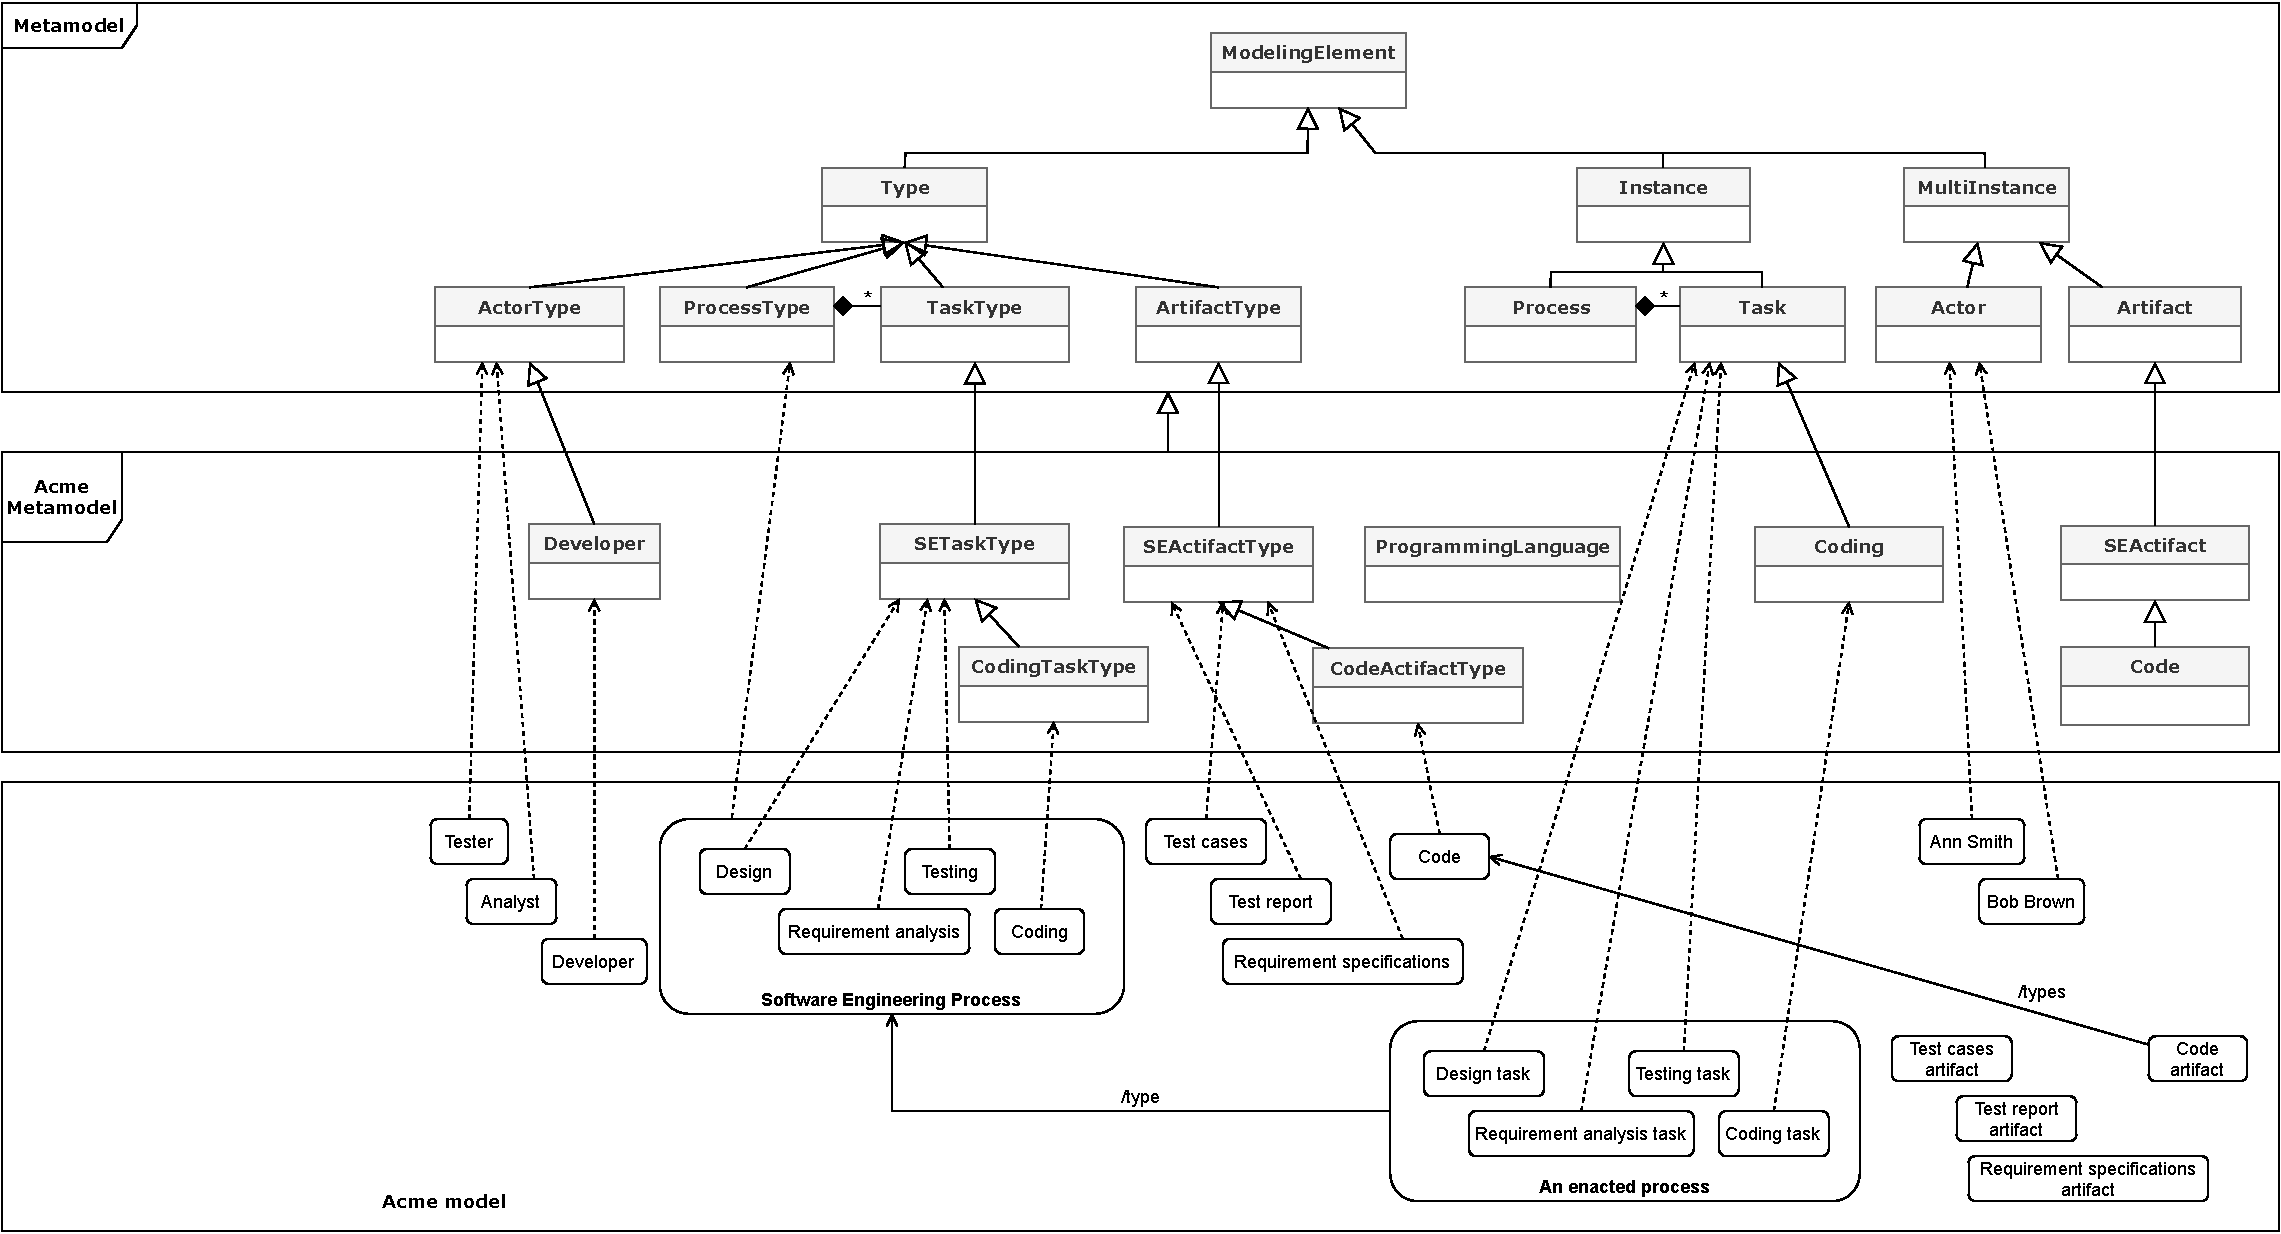
\includegraphics[width=1.0 \textwidth]{Figures/AcmeFullArchitecture.pdf}
     \caption{Acme software development process architecture}
    \label{fig:AcmeFullArchitecture}
\end{figure*}

\todo[inline]{Augmenter la taille des fontes de la figure \ref{fig:AcmeFullArchitecture}}
\todo[inline]{Ajouter les programming languages}

Figure \ref{fig:AcmeFullArchitecture} shows the full architecture capturing Acme software development process, with an instance of enacted \textit{Software Engineering Process}, and highlights all conceptual levels. Acme metamodel enriches base metamodel by offering specializing concepts: \textit{SETaskType} extending \textit{TaskType}, a more specialized concept \textit{CodingTaskType} extending \textit{SETaskType}, \textit{SEArtifactType} extending \textit{ArtifactType}, a more specialized concept \textit{CodeArtifactType} extending \textit{SEArtifactType}. Acme metamodel also defines task type \textit{Coding} as a specialized concept of \textit{Task}, and provides concept \textit{Developer} extending \textit{ActorType}. This metamodel is completed with \textit{ProgrammingLanguage} concept, defined as an enumeration (\textit{Java}, \textit{C}, \textit{COBOL}). All instances required to capture challenge use case are still defined in final Acme model itself instance of Acme metamodel. Instances are represented with rounded boxes and linguistic instantiation are represented with dashed connectors.

The \textit{Software Development Process} for Acme company is presented in the figure \ref{fig:AcmeSoftwareDevelopmentProcess} which is a screen-capture from the tooling developed in the context of the challenge and described in the next section. 

\begin{figure}
 \centering
    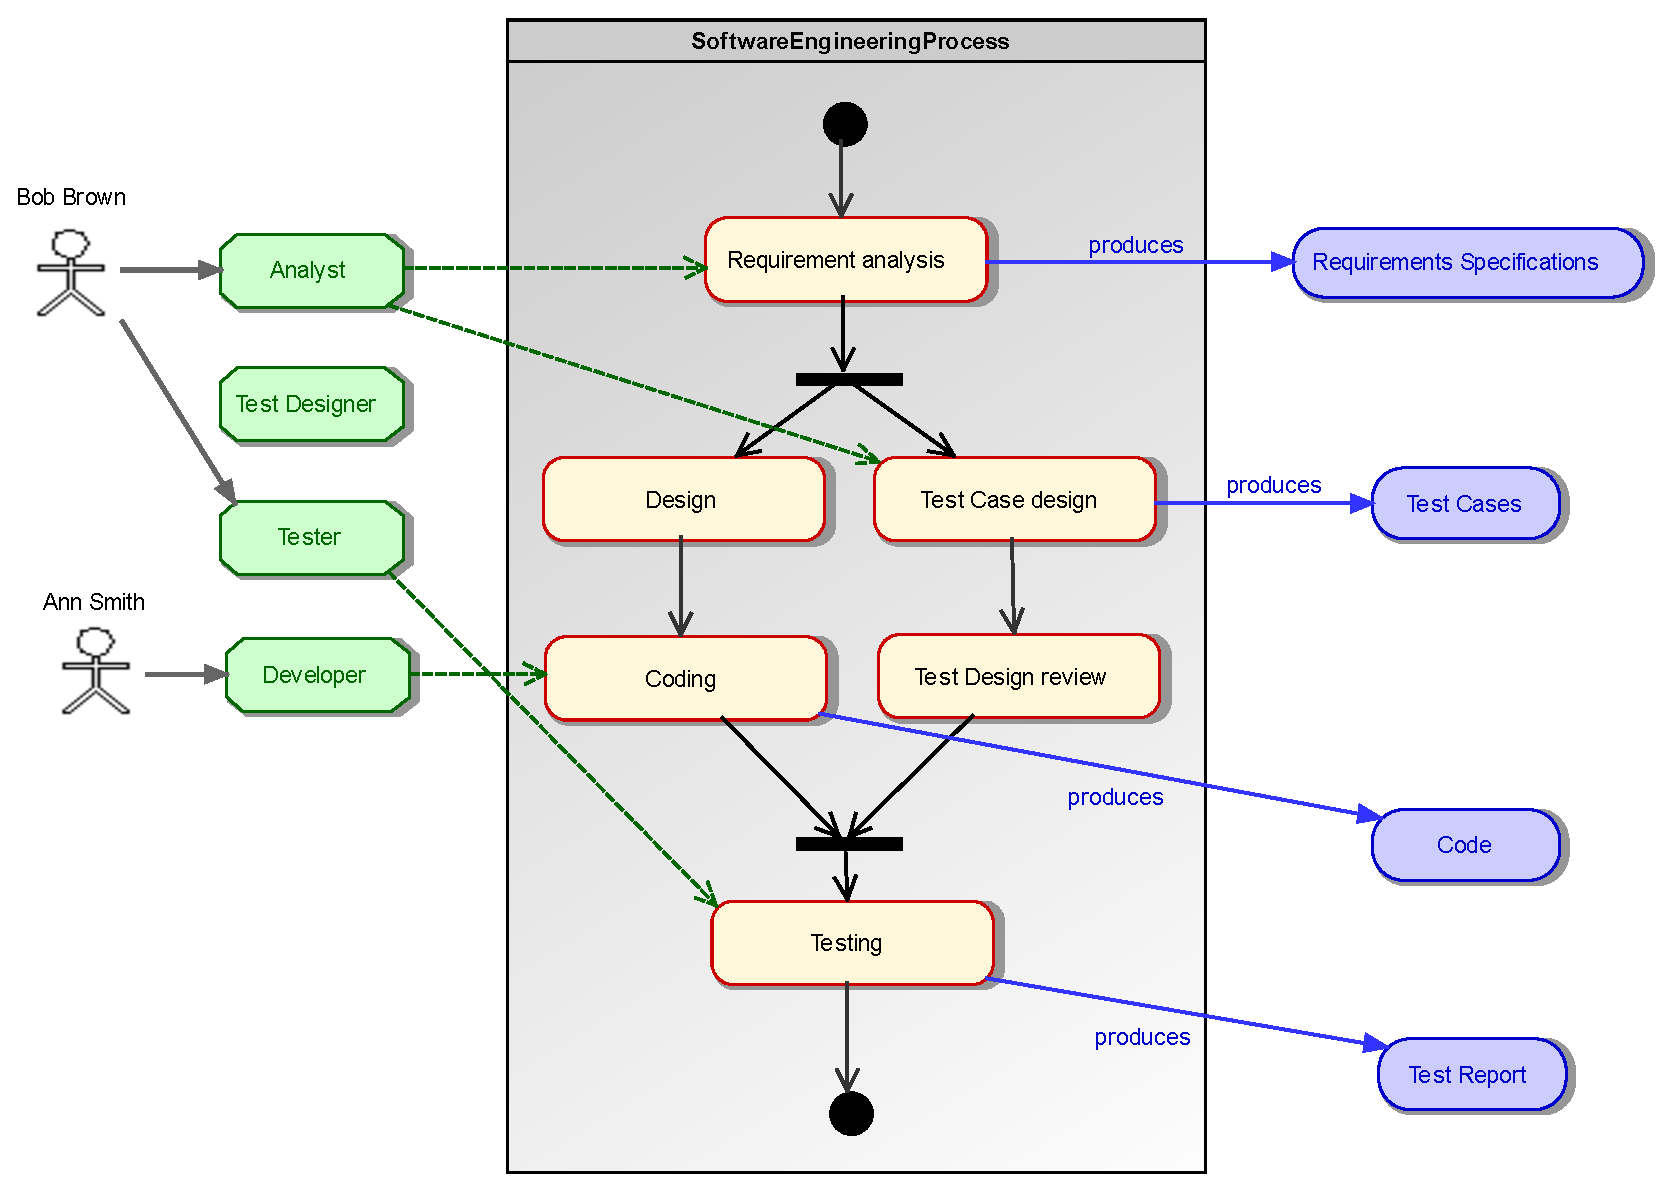
\includegraphics[width=1.0 \columnwidth]{Figures/SoftwareEngineeringProcessCroped.pdf}
     \caption{Acme software development process}
    \label{fig:AcmeSoftwareDevelopmentProcess}
\end{figure}

\textit{"Requirements analysis"} is defined as an instance of \textit{SETaskType}, \textit{Analyst} as an instance of \textit{ActorType} and \textit{Requirement specifications} as an instance of \textit{SEArtifactType}. \textit{"Requirements analysis"} instance defines property values \textit{producedArtifactTypes=\{Requirement specifications\}} and \textit{allowedActorTypes=\{Analyst\}} (\textbf{S1}). In the same way, \textit{"Test case design"} is defined as an instance of \textit{SETaskType}, marked as critical with property value \textit{isCritical=\{true\}}, and bound to \textit{Analyst} with \textit{allowedActorTypes} relation. \textit{"Test case design"} produces \textit{"Test cases"} defined as an instance of \textit{SETaskType}. The latter is used in "Test design review" (\textit{producedArtifactTypes} relation) (\textbf{S1} and \textbf{S13}, satisfied with \textbf{P9}). 

The capture of \textbf{S3} requirement is performed while defining \textit{Coding} as an instance of concept \textit{CodingTaskType} extending \textit{SETaskType} and defining a relation \textit{languages} to \textit{ProgrammingLanguage} with 1..* cardinality. \textit{newTask(String)} behavior overrides generic implementation while instantiating a \textit{Coding} concept, specializing \textit{SEArtifact}, as shown in following excerpt of FML code:

\begin{lstlisting}
concept CodingTaskType extends SETaskType {
  ProgrammingLanguage[1..*] languages;
  ...
  public Coding newTask(String name) { 
    return new Coding(name,this); 
  }
}    
\end{lstlisting}

\textit{Code} concept extends \textit{SEArtifact}, and defines a relation \textit{language} to \textit{ProgrammingLanguage} with single cardinality (\textbf{S4}). \textbf{S5} is more ambigous as task type \textit{Coding} defines one or more programming languages but produces code which is expressed in one language only. This requirement is captured through the redefinition of \textit{declaresRequiredProducedArtifacts()} where programming language should also match. 
\textbf{S6} is guaranteed though the \textit{language} relation defined in \textit{Code} and following invariant declared in \textit{Code}:  

\begin{lstlisting}
forEach (artifactType : types) {
  assert !(artifactType instanceof CodeArtifactType) | artifactType.doesImplement(languages)
}
\end{lstlisting}

\textit{Ann Smith} is the only one allowed to perform coding in COBOL (\textbf{S7}). This is implemented through the redefinition of \textit{newTask(String)} in \textit{CodingTaskType}:

\begin{lstlisting}
concept CodingTaskType extends SETaskType {
  ...
  public Coding newTask(String name) {
    Coding returned = new Coding(name,this); 
    if (languages.contains(ProgrammingLanguage.COBOL))
      returned.addToPerformingActors(getActor("Ann Smith"));
    return returned;
  }
}    
\end{lstlisting}

\textbf{S8} requirement is simply captured with the definition of \textit{Testing} instance of \textit{SETaskType}, \textit{Tester} instance of \textit{ActorType}, and \textit{Test report} instance of \textit{ArtifactType}.

\todo[inline]{requirement S9 non couvert pour le moment: compléter}


All software engineering artifacts defined in the context of Acme Software Engineering Process (figure \ref{fig:AcmeSoftwareDevelopmentProcess}) are all instances of \textit{SEArtifact} which defines both attributes \textit{responsible} (an \textit{Actor} instance), and \textit{versionNumber} (an \textit{integer} value), and thus fulfills \textbf{S10}. \textit{Bob Brown} is declared as an instance of \textit{Actor}, and references \textit{Analyst} and \textit{Tester} (\textit{ActorType} instances). He is also referenced by all instances of \textit{SETaskType} as the creator for related task types (\textbf{S11}).

\textbf{S12} is somehow ambiguous as it implies an implicit semantics regarding underlying business logic of process execution. We assume that all tasks may define an expected duration, which might be checked during process execution. This can be modeled through the addition of \textit{expectedDuration} attribute in \textit{TaskType}. Alternatively, this can be modeled through the definition of \textit{SETesting} concept, as a specialization of \textit{SETaskType}, and the instantiation of \textit{Testing} as an instance of \textit{SETesting}. The business logic expressed by \textbf{S12} requirement should be redefined in \textit{SETesting}.

\textbf{S13} requirement has been previously partially fulfilled. This must be completed with...

\todo[inline]{requirement S13 pas complètement couvert : compléter}

\subsection{Openflexo tooling}
\label{subsec:tooling}

Our solution is fully implemented within Openflexo tool. Both usecases have been modeled in the interactive design environment and are executable by the FML execution engine.

Base metamodel has been completed with some behaviors implementing execution semantic for executed processes. All tasks - instantiated from \textit{TaskType} for a given enacted process - manage a status which can be \textit{Not startable} (when not assigned to a performing actor or when required input artifacts are not available) , \textit{Startable}, \textit{Started}, \textit{Completable} (when all output artifacts are ready), \textit{Completed}). A \textit{Task} also manages a set of performing actors, a begin and end date, some used and produced artifacts. \textit{Gateways} business logic has also been implemented through the implementation of abstract \texttt{execute(Process)} behavior. Management of artifacts whose semantics follows rules defined in section \ref{sec:ProcessEnactment} (\textbf{P13}) has also been implemented.

We took advantage of model federation and the availability of diagramming features though the \textit{Diagramming TA} to implement two interactive graphical tools built on top of conceptual levels detailed in previous section. A first tool offers a graphical edition of a Process type, while the second tool offers enactment feature (the instantiation of a process from its process type), the ability within an enacted process to assign tasks to some actors, and the execution of this process with a graphical visualization.

\begin{figure*}
 \centering
     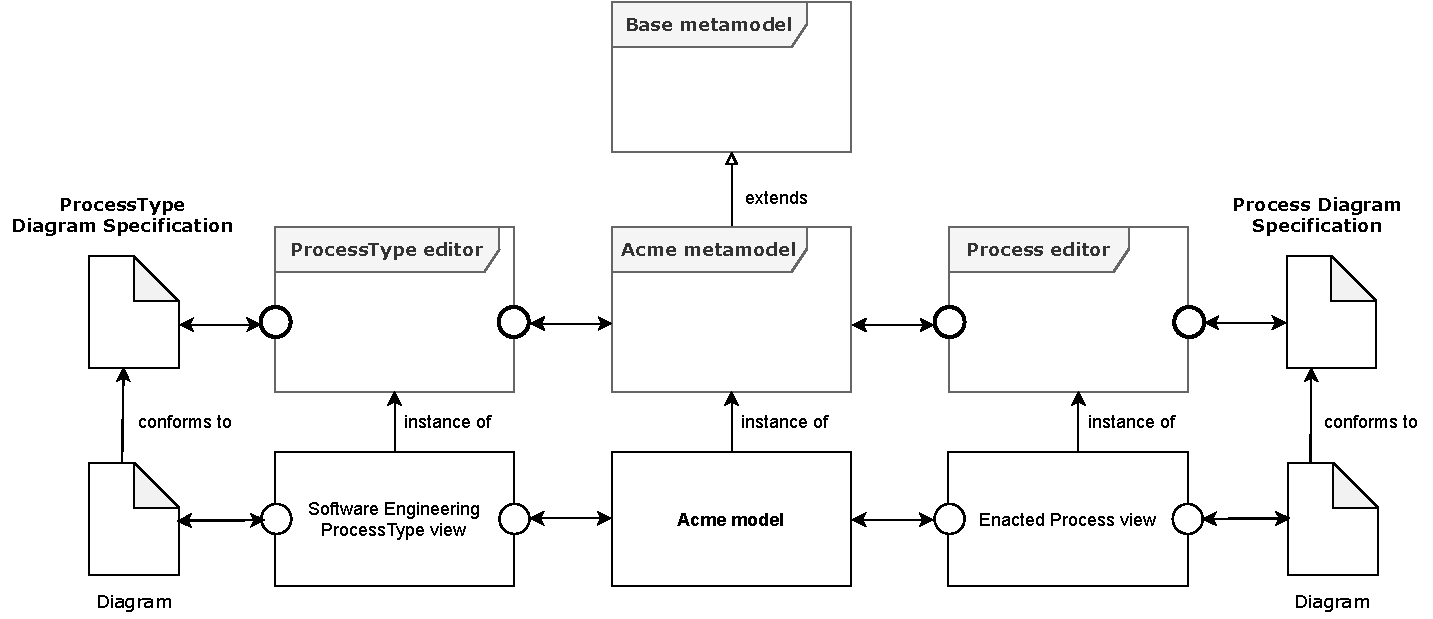
\includegraphics[width=0.9 \textwidth]{Figures/ToolingArchitecture.pdf}
     \caption{Tooling architecture}
    \label{fig:ToolingArchitecture}
\end{figure*}

Figure \ref{fig:ToolingArchitecture} shows the architecture of these two tools. Left of figure presents \textit{ProcessType graphical editor}. \textit{ProcessTypeEditor} is modeled as a \textit{VirtualModel} declaring two model slots (represented with bold circles). The first model slot references an instance of Acme metamodel, while the second model slot references an instance of diagram, conforms to the \textit{ProcessType diagram specification} (a diagram "metamodel" which defines and specify structure and graphical representations for edited items). While executed, this tool manages a graphical view for an instance of Acme metamodel (the \textit{Acme model}) and a specific \textit{ProcessType} instance. This tools allows to represent and edit a \textit{ProcessType}. One particular point should be noted regarding the highly reflective nature of FML and associated tooling : when drag and drop interactor is applied for a new item, the tool allows to choose the concept type to be instantiated (when a \textit{TaskType} is created for example, the user must choose the sub-concept of \textit{TaskType} to be selected - in Acme use case it can be \textit{SETaskTask} or \textit{CodingTaskType} or default value \textit{TaskType}). 

The other tool, called \textit{Enacted process graphical editor}, provides process edition and tasks assignations through a graphical visualization displaying process being executed. This tool is represented on the right side of the figure \ref{fig:ToolingArchitecture}. It follows the same architecture pattern as explicited for the \textit{ProcessType graphical editor}, with two model slots referencing both the model and a diagram. Process enactment is operated from a \textit{ProcessType}, and must be defined using a name identifying the newly instantiated process. All tasks are created from their \textit{TaskType} definition, and required assignments applies (if for example "Coding" \textit{TaskType} defines COBOL as output programming language, related task is automatically assigned to "Ann Smith"). All tasks get a status as well as a set of performing actors, a begin and end date, and used and produced artifacts. 

\todo[inline]{mettre ici le lien vers la page web qui montre la démo}



